\documentclass{beamer}
\usetheme{Copenhagen}
\usepackage{amsmath, amsthm, amsfonts, amssymb}
\usepackage{bbm}
\usepackage{hyperref}
\usepackage{cleveref}
\usepackage{mathrsfs}
\usepackage{listings}
\usepackage{color}

%% LaTeX stuff 
    % Definition of footnote
    \newcommand\blfootnote[1]{%
    \begingroup
    \renewcommand\thefootnote{}\footnote{#1}%
    \addtocounter{footnote}{-1}%
    \endgroup
    }

    % Transparency 
    \setbeamercovered{invisible}
    \setbeamercovered{%
    again covered={\opaqueness<1->{15}}}

    \newcommand\numberthis{\addtocounter{equation}{1}\tag{\theequation}}

%% Metadata
\author{Arnav Sood \\ \texttt{arnav.sood@ubc.ca}}
\title{Credit and Credibility}
\date{\today\blfootnote{\tiny Final project for ECON 514 (Winter 2019), ``Information and Incentives.'' Thanks to Vitor Farinha Luz, Jesse Perla, and Xiaojun Guan for their support and many helpful comments. All errors are my own.}}

\begin{document}
\maketitle

\begin{frame}
    \frametitle{Motivation}
    Producers of public information are subject to economic incentives. \pause
    \begin{itemize}[<+>]
        \item Setting: \textbf{Credit Ratings Agencies (CRAs)}, who earn fees from the firms they rate (so-called ``issuer-pays model.'')  
        \item Incentives: 
        \[ \max\limits_{\text{price, ratings}} \mathbb{E} \sum_{t = 0}^\infty \beta^t \text{profits} \] 
        \item Ratings is a choice variable! 
        \item \textbf{Empirics} Gillette et al. (2018): Unexpected positive shock to ratings improves CRA market share and profits. 
        \item \textbf{Empirics} 2008 Recession?
    \end{itemize}
\end{frame}

\section{Model Ingredients}

\begin{frame}
    \frametitle{Our Model (English)}
    One-shot CRA choosing prices and ratings for a continuum of firms, with a lower bound on ratings informativeness. \pause 
    \begin{itemize}[<+>]
        \item Firms: $i \in [0, 1]$, with $\theta_i \in \{H, L\}$. Have outside options contingent on type: $\omega_i \sim F_\theta$. 
        \item Capital Market: Invests in any firm which gets a good signal (WLOG, it can be shown there are two signals), so long as there's a minimum ``precision.'' 
        \item CRA: Forward-looking to market behavior and firm entry decisions, chooses a public mechanism $(p, \phi)$, where $\phi \in \mathbb{R}$ summarizes the ratings policy. 
    \end{itemize}
\end{frame}

\begin{frame}
    \frametitle{Our Model (Firms)}
    \begin{itemize}[<+>]
        \item Mass-one continuum indexed by $i \in [0, 1]$, types $\theta_i \in \{H, L\}$ (``High,'' ``Low.'')
        \item Realized types are unimportant, since model is solved in expectation. Common prior: $\Pr[\theta_i = H] = \lambda$. 
        \item Outside options follow type-contingent distributions $F_\theta$ on $[\underline{\omega_\theta}, \overline{\omega_\theta}]$. 
        \item Mechanistically solve: 
        \begin{equation}
            V_i \equiv \max \{\omega_i, \mathbb{E} U(\theta) - p \}
            \label{firm-objective}
        \end{equation}
    \end{itemize}
\end{frame}

\begin{frame}
    \frametitle{Our Model (Capital Market)}
    \begin{itemize}[<+>]
        \item Assigns outcomes to firms according to a simple cutoff rule: 
        \begin{equation}
            U: \theta \mapsto R \underbrace{\mathbbm{1}_{\lambda^o(\theta) \geq \underline{\lambda}, \theta = h}}_{\text{Binary investment decision}}    
            \label{market-objective}
        \end{equation}
        \item What's required for investment? 
    \end{itemize} \pause
    \begin{enumerate}
        \item A positive signal $h$. \emph{and}
        \item A minimum posterior $\Pr[\theta_\text{firm} = H | \text{signal} = h] \geq \underline{\lambda}$ 
    \end{enumerate}
\end{frame}

\begin{frame}
    \frametitle{Our Model (CRA)}
    \begin{itemize}[<+>]
        \item Assume (WLOG) that ratings space $\xi \equiv \{h, l\}$. 
        \item Can be shown that $H \mapsto h$ always (``why hide peaches?'') So ratings decision is map $f: L \mapsto \Delta(\xi)$.
        \item Can summarize $f$ by $\phi \in \mathbb{R}$ s.t. $\phi \equiv \Pr[\theta_i = L, \xi_i = h]$.
        \item Objective is then: 
        \begin{equation}
            \max\limits_{p \geq 0, \phi \in [0, 1]} p \{F_L(\phi R - p)(1 - \lambda) + F_H(R - p)\lambda\}
            \label{CRA-objective}    
        \end{equation} s.t. the constraint in \eqref{market-objective} is satisfied. 
        
        \hspace{1 em} \\ 

        This objective is \textbf{forward-looking}, in that it incorporates optimality conditions for firms and the market. 
    \end{itemize} 
\end{frame}

\begin{frame}
    \frametitle{Our Model (Timing)}
    \begin{enumerate}[<+>]
        \item The CRA chooses a scheme $m \equiv (p, \phi)$ according to the common prior $\lambda$ about the share of high-type firms, in order to solve \eqref{CRA-objective}.
    
        \item Firms observe $(p, \phi)$, and make entry decisions according to \eqref{firm-objective}. Denote the proportion of firms of type $\theta$ which decide to buy ratings as $e_\theta$ (i.e., the mass of high entrants is $e_H \lambda$.)
        
        \item The market observes $\{(p, \phi), e_H, e_L\}$, and mechanistically executes the investment rule in \eqref{market-objective}.    
    \end{enumerate}
\end{frame}

\begin{frame}
    \frametitle{Equilibrium Ingredients}
    A CRA policy $(p, \phi)$, entry decisions $e_H, e_L$, and a market ratings policy (call it $\pi: \xi \to \{0, R\}$) s.t. ...
    \begin{enumerate}
        \item $\pi(\cdot)$ solves the market's problem, \eqref{market-objective}.
        \item Entry decisions $e_H, e_L$ maximize the firm objective \eqref{firm-objective}.
        \item CRA actions $(p, \phi)$ maximize the CRA objective \eqref{CRA-objective}.
        \item CRA actions are optimal in expectation, policies $e_H, e_L$ are forward-looking best-responses, and market outcomes $\pi(\cdot)$ are updated in a Bayes-plausible way.
    \end{enumerate}
\end{frame}

\begin{frame}
    \frametitle{Our Model (Caveats)}
    Before proceeding with an analysis of this model, it's worth examining its implicit assumptions. 

\begin{enumerate}[<+>]
    \item \textbf{No Transfer Payments:} Maybe $L$-type firms (who may have more to gain from a high credit rating) might pay more for a good rating. This is ruled out by our flat price $p$.
    
    \item \textbf{No Outside Information:} The only source of information is the single CRA. In practice, there is a competitive market for information\footnote{See, e.g., Veldkamp (2006a)}, which may discipline the CRA.
    
    \item \textbf{No Inside Information:} Likewise, we do not allow firms to generate their own information (e.g., in reality a high-type firm may decide to seek debt financing instead of equity financing.)
    
    \item \textbf{No CRA Competition:} In practice, the credit-ratings industry is an oligopoly and not a monopoly.
\end{enumerate}
\end{frame}

\section{Analytical Results}

\begin{frame}
    \frametitle{Backwards Induction}
    \begin{enumerate}[<+>]
        \item Calculate $\lambda^o(h|p, \phi, e_H, e_L)$, or the posterior about type conditional on a high signal.
        \item Given $\uparrow$, solve for $e_H|(p, \phi), e_L|(p, \phi)$. 
        \item Given $\uparrow$, solve for $p, \phi$.
    \end{enumerate}
\end{frame}

\begin{frame}
    \frametitle{Market's Posterior}
    \begin{enumerate}[<+>]
        \item Start with \emph{inflow prior}, $\Pr[\theta_i = H | \text{entry}]$:
        \begin{equation}
            \label{inflow-prior}
            \lambda^I \equiv \frac{e_H \lambda}{e_H \lambda + e_L (1 - \lambda)}
        \end{equation}
        \item This implies; 
        \begin{equation}
            \lambda^o(h) = \frac{\lambda^I}{\lambda^I + (1 - \lambda^I)\phi}
        \end{equation} 
        \item Which can be rewritten in terms of raw policies: 
        \begin{equation}
            \label{lambda-o-final}
            \lambda^o(h) = \frac{e_H \lambda}{e_H \lambda + \phi e_L (1 - \lambda)}
        \end{equation}
    \end{enumerate}
\end{frame}

\begin{frame}
    \frametitle{Entry Policies}
    \begin{itemize}[<+>]
        \item In an interior solution, $H$ types can expect reward $R$ with probability 1, and $L$ types can expect it with probability $\phi$. 
        \item Gives us the following: 
        \begin{align}
            e_H &= F_H(R - p) \label{high-entry} \\ 
            e_L &= F_L(\phi R - p) \label{low-entry}
        \end{align}
    \end{itemize}
\end{frame}

\begin{frame}
    \frametitle{Market Credibility Constraint}

Can rewrite $\lambda^o(h) \geq \underline{\lambda}$...

\begin{align*}
    \lambda^o(h) &\geq \underline{\lambda} \\ 
    \frac{e_H \lambda}{e_H \lambda + \phi e_L (1 - \lambda)} &\geq \underline{\lambda} \hspace{5 em} \text{by \eqref{lambda-o-final}} \\ 
    e_H \lambda (1 - \underline{\lambda}) &\geq \phi e_L \underline{\lambda} (1 - \lambda) \\ 
    \phi &\leq \frac{e_H \lambda (1 - \underline{\lambda})}{e_L \underline{\lambda} (1 - \lambda)} \label{MC-cons}\numberthis
\end{align*} \pause 

This last constraint (which we call the \textbf{Market Credibility} constraint, or (MC)) can be interpreted as a sort of discipline on the CRA's dishonesty $\phi$. It says that the CRA cannot lie so much that the market ceases to invest in any firms. 
\end{frame}

\begin{frame}
    \frametitle{Raters' Lagrangian}
We wish to solve \eqref{CRA-objective} subject to \eqref{MC-cons}.

Write the Lagrangian: 

\begin{align*}
    \mathscr{L} &\equiv p \{ F_H (R - p)\lambda + F_L(\phi R - p)(1 - \lambda)\} \label{Lagrangian} \numberthis \\ 
    &- \mu(\log \phi + \log F_L(\phi R - p) - \log F_H(R - p) - \log \tau)
\end{align*}
\end{frame}

\begin{frame}
    \frametitle{FOC $p$}

    \begin{align*}
        0 &= F_H (R - p)\lambda + F_L(\phi R - p)(1 - \lambda) \numberthis \label{FOC-p}  \\ 
        &- p\left(f_H(R - p)\lambda + f_L(\phi R - p)(1 - \lambda)\right)   \\ 
        &+ \underbrace{\mu \left(\frac{f_L (\phi R - p)}{F_L (\phi R - p)} - \frac{f_H(R - p)}{F_H(R - p)}\right)}_{\text{\emph{Composition} of customer pool changes!}}
    \end{align*}
\end{frame}

\begin{frame}
    \frametitle{FOC $\phi$}

    \begin{equation}
        \label{FOC-phi}
        \underbrace{\phi R (1 - \lambda)f_L(\phi R - p)}_{\text{Marginal return to $L$-type firms}} = \mu \left(\frac{1}{p} + \underbrace{\frac{\phi R}{p} \cdot \frac{f_L(\phi R - p)}{F_L(\phi R - p)}}_{\text{something like $\Delta \%$}}\right)
    \end{equation}
\end{frame}

\begin{frame}
    \frametitle{Analytical Propositions}

    Note: Full proofs are up on \href{https://github.com/arnavs/credit-pricing}{\color{blue} GitHub}.

    \begin{itemize}[<+>]
        \item \textbf{Existence:} Objective is continuous, can be shown that feasible set is compact. So Weierstrass EVT shows existence.
        \item \textbf{No Truth-Telling:} Will always be some entry. Since constraint is continuous, can always do a little better without exhausting slack.
        \item \textbf{Constraint Always Binds:} By Fermat, need (a) non-differentiable point, (b) a stationary point, or (c) a boundary point. Assume $F_H, F_L \in C^1$, so no (a). $\frac{\partial}{\partial \phi}$ of objective \eqref{CRA-objective} is (subject to assumptions) nonzero. So, must be a boundary.
    \end{itemize}

\end{frame}

\section{Comparative Statics}

\begin{frame}
    \frametitle{Vanilla Model}
    \begin{columns}
        \begin{column}{0.18\textwidth}
            \begin{itemize}
                \footnotesize
                \item $R = \frac{1}{2}$    
                \item $\lambda = \frac{1}{3}$.
                \item $\underline{\lambda} = \frac{1}{2}$.
                \item $\omega_i \sim U[0, 1]$.
                \item $\omega_i \sim U[0, 1]$.
            \end{itemize}        
        \end{column}
        \begin{column}{0.88\textwidth}
            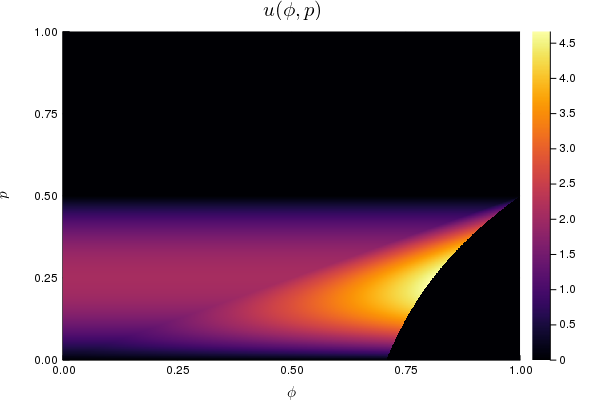
\includegraphics[scale=0.48]{vanilla.png}
        \end{column}
    \end{columns}
\end{frame}

\begin{frame}
    \frametitle{Adjusting $\lambda$}
    \begin{columns}
        \hspace{-1 cm}\begin{column}{0.5\textwidth}
            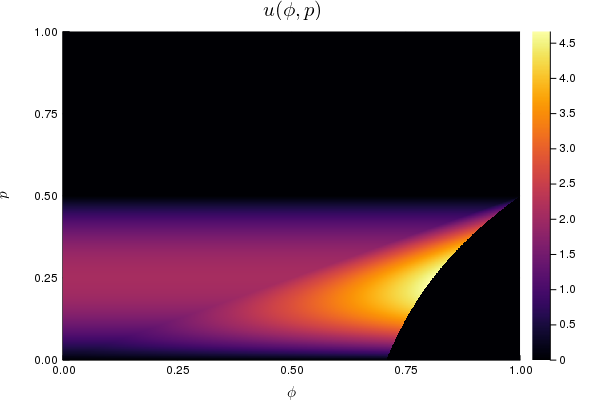
\includegraphics[scale=0.3]{vanilla.png}
        \end{column}
        \begin{column}{0.5\textwidth}
            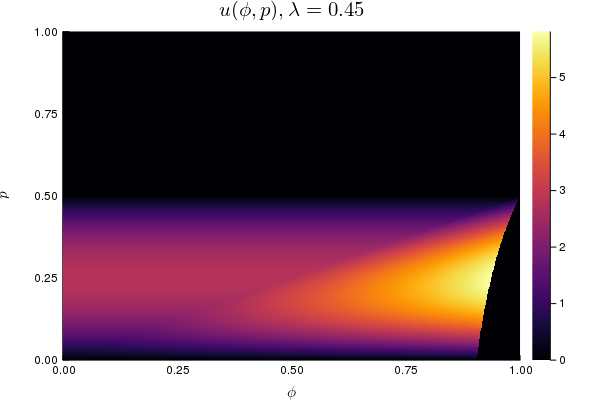
\includegraphics[scale=0.3]{small_lambda.png}
        \end{column}
    \end{columns}
\end{frame}

\begin{frame}
    \frametitle{Adjusting $\underline{\lambda}$}
    \begin{columns}
        \hspace{-1 cm}\begin{column}{0.5\textwidth}
            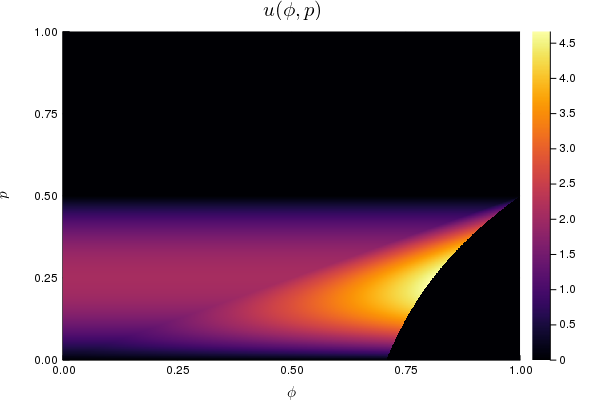
\includegraphics[scale=0.3]{vanilla.png}
        \end{column}
        \begin{column}{0.5\textwidth}
            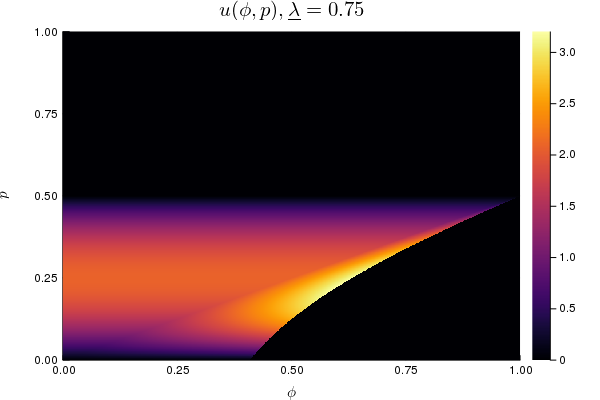
\includegraphics[scale=0.3]{high_lambda_bar.png}
        \end{column}
    \end{columns}
\end{frame}

\begin{frame}
    \frametitle{Adjusting $R$}
    \begin{columns}
        \hspace{-1 cm}\begin{column}{0.5\textwidth}
            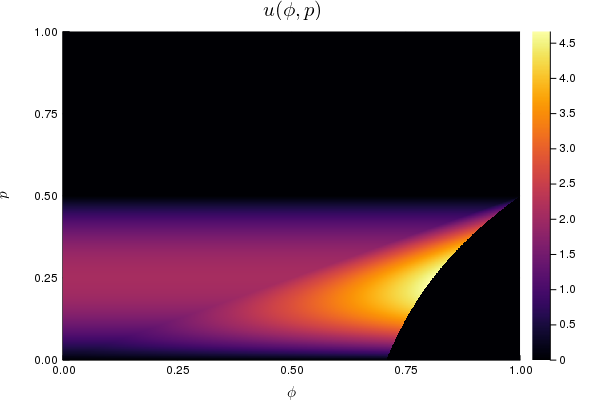
\includegraphics[scale=0.3]{vanilla.png}
        \end{column}
        \begin{column}{0.5\textwidth}
            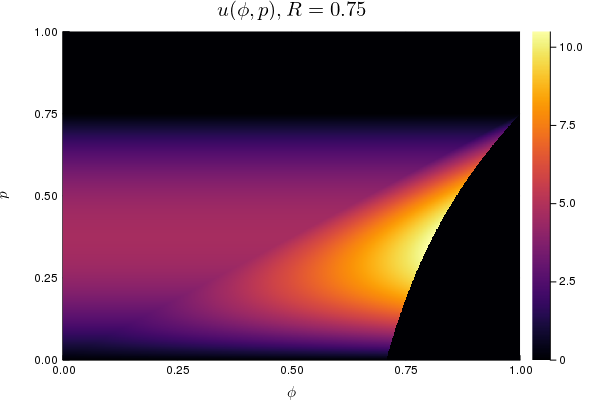
\includegraphics[scale=0.3]{high_R.png}
        \end{column}
    \end{columns}
\end{frame}

\begin{frame}
    \frametitle{Adjusting $\lambda$ (Degenerate)}
    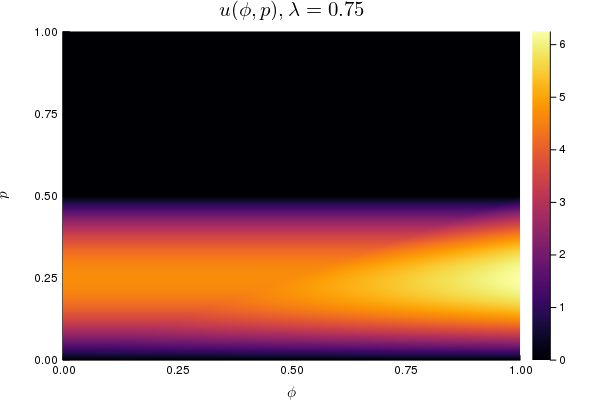
\includegraphics[scale=0.5]{high_lambda.png}
\end{frame}

\begin{frame}
    \frametitle{Adjusting $F_L$ (Degenerate)}
    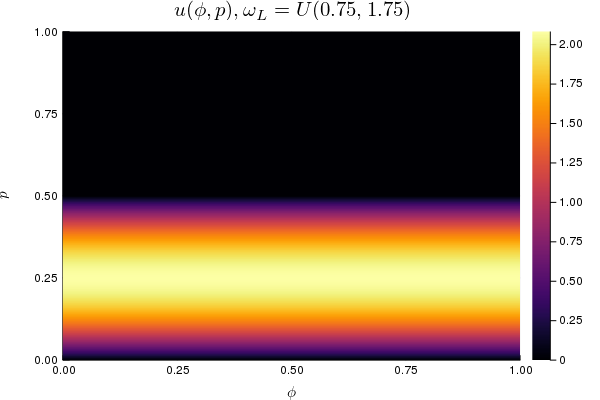
\includegraphics[scale=0.5]{high_L.png}
\end{frame}


\section{Wrap-Up}

\begin{frame}
    \frametitle{Wrap-Up}
    \begin{itemize}
        \item Solving the one-shot (pricing, ratings) problem gives us standard monopoly FOCs, with an additional term.
        \item There is a clean closed form for the \textbf{market credibility constraint} \eqref{MC-cons}, which always binds.
        \item Comparative statics reveal a number of outcomes, depending on parameters.
        \item Code up at  \url{https://github.com/arnavs/credit-pricing}
    \end{itemize}
\end{frame}

\begin{frame}
    \frametitle{Questions}
    \scriptsize 
    FAQ...
    \begin{itemize}
        \item \emph{Isn't your model unrealistic/overly stylized? Why is it useful?} \\ 
        A: The model helps illustrate the simultaneous role of CRA prices (as prices, and also as a ``lever'' to impact the ratings pool.) 

        \item \emph{You mentioned some caveats. Can these be relaxed?} \\ 
        A: The (no outside information) and (CRA is a monopoly) ones can be jointly loosened by modeling CRAs as symmetric price-makers. Firms can also produce their own signals, which would replace $\pi: \xi \to \{0, R\}$ with $\pi: \xi \times \Gamma \to \{0, R\}$. 

        \item \emph{How would one generalize beyond the one-shot binary case?} \\ 
        A: We could make the model a finite or infinite horizon model by incorporating a reputational term to the CRA objective \eqref{CRA-objective}, as we've seen in class. And/or partition the $n$-dimensional ratings space.

        \item \emph{Data?} \\ 
        A: We haven't used any, but there is lots of data on credit ratings and outcomes, which could conceivably be used to calibrate a model of strategic behavior by CRAs. This isn't a \emph{sui generis} area of research\footnote{See, e.g., Xia (2011), who studied over 70K ratings.}
    \end{itemize}
\end{frame}

\end{document}
